\documentclass{IEEEtran}

\usepackage{graphicx}
\graphicspath{{images/}}
\usepackage{algorithm2e}

%Title 
\title{Hadoop add-on API for Advanced Content Based Search \& Retrieval}
\author{Kshama Jain, Aditya Kamble, Siddhesh Palande, Rahul Rao\\ Guided by: Prof. Shailesh Hule\\ Department of Computer Engineering\\ Pimpri Chinchwad College of Engineering, Pune}

\begin{document}
\maketitle

%Abstract
\begin{abstract}
Unstructured data like doc, pdf is lengthy to search and filter for desired information. We need to go through every file manually for finding information. It is very time consuming and frustrating. We can use features of big data management system like Hadoop to organize unstructured data dynamically and return desired information. Hadoop provides features like Map Reduce, HDFS, HBase to filter data as per user input. Finally we can develop Hadoop Addon for content search and filtering on unstructured data.
\end{abstract}

\begin{IEEEkeywords}
Hadoop, Map Reduce, HBase, Content Based Retrieval.
\end{IEEEkeywords}

\section{Introduction}
\subsection{Hadoop}
Hadoop is an open-source software framework written in Java for distributed storage and distributed processing of very large data sets on computer clusters built from commodity hardware. Commodity computing, or commodity cluster computing, is the use of large numbers of already-available computing components for parallel computing, to get the greatest amount of useful computation at low cost. All the modules in Hadoop are designed with a fundamental assumption that hardware failures (of individual machines, or racks of machines) are commonplace and thus should be automatically handled in software by the framework. The core of Apache Hadoop consists of a storage part (Hadoop Distributed File System (HDFS)) and a processing part (Map Reduce). Hadoop splits files into large blocks and distributesthem amongst the nodes in the cluster.

\subsection{HDFS}
The Hadoop Distributed File System (HDFS) is a distributed file system designed to run on commodity hardware. HDFS is highly fault-tolerant and is designed to be deployed on low-cost hardware. HDFS provides high throughput access to application data and is suitable for applications that have large data sets.

\subsection{MapReduce}
A MapReduce program is composed of a Map() procedure(method) that performs filtering and sorting and a Reduce() method that performs a summary operation. The MapReduce System run the various tasks in parallel, managing all communications and data transfers between the various parts of the system.

\subsection{HBase}
HBase is a data model that is similar to Google’s big table designed to provide quick random access to huge amounts of structured data. This tutorial provides an introduction to HBase, the procedures to set up HBase on Hadoop File Systems, and ways to interact with HBase shell. It also describes how to connect to HBase using java, and how to perform basic operations on HBase using java.

\subsection{Current System}
Taks like assignments, taking notes from text books and reference books on particular topic, topics for presentation need deep reading and need to go through every document manually just to find relevant content on given topic.
Currently present systems are only searching based on document title, author, size, and time but not on content. So to do content based search on big data documents and large text data Haddop framework can be used.

\subsection{Content Based Approach}
Manually filtering from any kind of unstructured data like PDF is tedious and time consuming, we are developing API for Hadoop finding relevant information from large sets and retrieving the same is main concern. So using Hadoop Big Data management framework consist of HDFS, MapReduce, and HBase, we are developing content based search on PDF documents to solve real life problem. So this is basic motivation for the project.

\section{Proposed System}
This system shall retrieve the required contents of files which are in an unstructured format containing huge amount of Data like e-books in a digital library where the number of books are present in thousands. The scope here is initially limited to PDF files which may be expanded to other unstructured formats like ePUB, mobi. The input is provided to the system API in the form of search query which will be firstly filtered to find the important expression as a query to the API which will return the important content to the user in the form of paragraph or text highlighted using the power of distributed computing. The particular page or the Entire book itself can be downloaded by the Library users if the content is satisfied else the search continues for finding relevant content 

\begin{figure}[h]
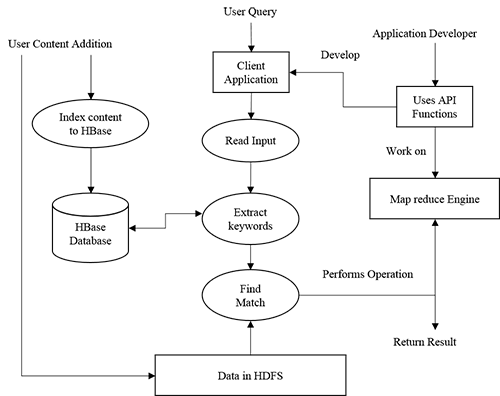
\includegraphics{data_flow}
\caption{Data Flow Diagram}
\end{figure}

\begin{figure}[h]

\includegraphics{activity_diagram}
\caption{Activity Diagram}
\end{figure}

\begin{algorithm}[h]
\begin{enumerate}
\item Take Input Query from User
\item Use the Suffix Stripping Algorithm to remove English Suffixes like 'ed','ing',' ' 's ' to extract keywords
\item Match keywords with Documents' metadata present in Hbase and filter the documents to be searched.
\item Apply Searching Algorithm based on map-reduce operations like keyword count,positions.
\begin{itemize}
\item Open the PDF
\item Distribute the text using map operation.
\item combine the results with reduce operations.
\end{itemize} 
\item Sort the documents which are returned by Searching w.r.t keyword count and relevance.
\item Depending on API methods return the result with 
\begin{itemize}
\item Paragraph
\item Whole Page
\item Current and Previous Page
\end{itemize}
\end{enumerate}
\caption{Content Based Search Algorithm}
\end{algorithm}

\begin{algorithm}[h]
\SetAlgoLined
Meta-data Extraction Service
\begin{enumerate}
\item Take the input pdf files from user
\item Check if corrupt
\item Upload the file into the Hadoop Distributed Filesystem
\item Run the Metadata Extracting Algorithm using the Map Reduce Engine.
\item Extract the Bibliography and Index Contents of each and every document (if present) and related keywords.
\item Store it in the HBase as metadata.
\item This metadata will be used by map reduce engine to search and retrieve data from relevant document inside HDFS using keyword relative custom partitioning.
\item Return the result to the search API
\item Stop
\end{enumerate}
 \caption{Meta-data Extraction Service Algorithm}
\end{algorithm}


\subsection{Document Metadata}
Searching and retrieving information from data inside HDFS. Hadoop Map Reduce operations will be used to perform key value pair generation and depend upon result information is searched. 
\paragraph{}
Here, data is documents in PDF ( Portable Document Format ) format. These documents are stored on HDFS - Hadoop Distributed File System. These documents are considered as raw data. These documents can have properties like
\begin{itemize}
\item Name
\item Size
\item Date
\item Author
\end{itemize}
\paragraph{}
Document meta data is also maintain in HBase distributed database. It has attributes like
\begin{itemize}
\item Content Keywords
\item Index Keyword
\item Document Keywords
\end{itemize}
This information will be useful to filter documents before performing content based  searching operations.

\section{Applications}
\begin{itemize}
\item Content based search and retrieval on
\begin{enumerate}
\item Digital library books 
\item Conference Papers
\item Private Authorities
\item Government Authorities
\item Unstructured text files
\end{enumerate}

\item This API can be used to develop above functionality on platforms like
\begin{enumerate}
\item Web Application
\item Android Application
\item Standalone Application
\item Command Line Interface Application
\end{enumerate}

\end{itemize}

\section{Future Scope}
Extending our API further to read scanned text copies and retrieve the data from them would solve further advanced issues. This API again can be extended further to work with Image processing so that it may find a relevant information from the digital images for the end- users.

\section{Conclusion}
This API would be favorable for many large organizations like Large-scale Industries and Educational institutes, Power-Grids, Air-lines, Government Offices and many others working with and producing Big-Data to retrieve data in an efficient and a very cost effective way.
Thus we can use this API in Hadoop to reduce manual efforts and bring advance content based search and retrieval

\begin{thebibliography}{7}
\bibitem {R1} Lars George, "HBase: The Definitive Guide", 1st edition, O'Reilly Media, September 2011, ISBN 9781449396107


\bibitem {R2} Tom White, "Hadoop: The Definitive Guide", 1st edition, O'Reilly Media, June 2009, ISBN 9780596521974

\bibitem {R3} Apache  Hadoop HDFS homepage http://hadoop.apache.org/hdfs/

\bibitem {R4} Mehul Nalin Vora ,"Hadoop-HBase for Large-Scale Data",Innovation Labs,PERC,ICCNT Conference

\bibitem {R5} Yijun Bei,Zhen Lin,Chen Zhao,Xiaojun Zhu ,"HBase System-based Distributed Framework for Searching Large Graph Databases",ICCNT Conference


\bibitem {R6} Seema Maitrey,C.K."Handling Big Data Efficiently by using Map Reduce Technique",ICCICT

\bibitem {R7} Maitrey S, Jha. An Integrated Approach for CURE Clustering using Map-Reduce Technique. In Proceedings of Elsevier,ISBN 978-81- 910691-6-3,2 nd August 2013.


\end{thebibliography}

\end{document}